\chapter{Analysis}

In this chapter, I will present and analyze the data made available by the MCP in the three documents \ttt{E2 - NW-NM DMA Service Instance}, \ttt{E2 - NW-NM REST Service Technical Design}, and \ttt{E2 - NW-NM Service Specification}, which represent all data, made available to me. Furthermore, I will explain the necessity of testing the MCP, as well as present a description of a favorable model structure. 

\section{Data}

To provide a holistic description of a service instance, three documents are necessarily provided. Below are the descriptions of the documents with the service instance \ttt{E2 - NW-NM DMA} as an example.
\begin{description}
	\item[E2 - NW-NM DMA Service Instance]\ \\
	The purpose of this service instance document and its xml-defined counterpart is to describe a DMA instance of the REST-based technical design of the MW- NM service specification, according to the guidelines given in the Service Description Guidelines.
	\item[E2 - NW-NM REST Service Technical Design]\ \\
	The purpose of this service technical design document and its xml-defined counterpart is to describe a REST-based technical design of the MW-NM service specification, according to the guidelines given in the Service Description Guidelines.
	\item[E2 - NW-NM Service Specification]\ \\
	The purpose of this service specification document and its xml-defined counterpart is to provide a holistic overview of the MW-NM service and its building blocks in a technology-independent way, according to the guidelines given in the Service Description Guidelines.
\end{description}
Of the three documents, only the last, \ttt{Service Specification} is to be used to describe specifications of the service, and as such only this will be studied closer.
\section{Service Specification grammar}
The service specification document is constructed using a general xml-format. The grammar of the document can be seen in Listing \ref{fig:sSpecFull} as well as in Listing \ref{fig:sSpecRed}, while the latter is in a severely reduced and generalized form.
\TODO{evt læg i appendix og referer til relevante bidder.
meget mere om listings.
Håbløst placering af tekst/figurer}


\begin{figure}
	\centering
	\begin{lstlisting}[keywordstyle={}]
ServiceSpecificationSchema ::= specifications

specifications ::= spec specifications
     | $\e$
     
spec ::= name
     | status
     | id
     | version
     | description
     | keywords
     | isSpatialExclusive
     | authorInfos
     | requirements
     | serviceDataModel
     | serviceInterfaces
     
authorInfos ::= authorInfo authorInfos
     | $\e$

authorInfo ::= aSpec authorInfo
     | $\e$

aSpec ::= id
     | name
     | description
     | contactInfo

requirements ::= requirement requirements
     | $\e$

requirement ::= rSpec requirement
     | $\e$

rSpec ::= id
     | name
     | text

serviceDataModel ::= definitionAsXSD

definitionAsXSD ::= $\e$

serviceInterfaces ::= serviceInterface serviceInterfaces
     | $\e$

serviceInterface ::= siSpec serviceInterface
     | $\e$

siSpec ::= name
     | description
     | dataExchangePattern
     | operations

operations ::= operation operations
     | $\e$

operation ::= oSpec operation
     | $\e$

oSpec ::= name
     | description
     | returnValueType
     | parameterTypes

returnValueType ::= typeReference


parameterTypes ::= parameterType parameterTypes
     | $\e$

parameterType ::= ptSpec parameterType
     | $\e$

ptSpec ::= typeReference
	\end{lstlisting}
	\caption={Full parser grammar of Service Specification Schema.}
	\label{fig:sSpecFull}
\end{figure}

\begin{figure}
	\centering
	\begin{lstlisting}[keywordstyle={}]
ServiceSpecificationSchema ::= specifications

specifications ::= spec specifications
     | $\e$
     
spec ::= specifications
     | spec
     | $\e$

spec ::= string
	\end{lstlisting}
	\caption{Reduced parser grammar of Service Specification Schema.}
	\label{fig:sSpecRed}
\end{figure}

As mentioned above, the service specification is to be used to verify the behavior of the maritime service from a technical stand point. At the moment, the xml-document provides a technical description of its corresponding maritime service, but the most commonly used expression method is free text. As this is a very non-technical design choice, a large portion of the obvious technical advantages, provided by the xml-format are lost. 

As it is possible to utilize free text though the use of natural language processing \cite{nlp}, no modifications are strictly necessary, however even with utilization of such or similar method, implementation hereof would be unstable in terms of usability. This is due to the fact that free language formulation varies at an unforeseeable degree, and as such creating uniform model based on this would add a great layer of complexity.

For a more sustainable solution to the problem, see Section \ref{sec:Updated Data}.

The xml-version of the service specification can be found in appendix \ref{sec:E2 - NW-NM Service Specification}.

\section{Testing the MCP}

The core principle in the MCP is to restructure and streamlining maritime software sharing in a manner that can be done the world over, and the very nature of this statement dictates that the platform must be highly scalable. This adds the necessity of running quality-checks on all of the maritime services that are uploaded to the platform. To accommodate this issue, model-based testing immediately seems like the obvious solution, as this technique covers most of the required desired functionality. If implemented satisfyingly, a model-based testing suite for the MCP would be able to
\begin{enumerate}
	\item Present or verify behavior of maritime services.\\
	There are many obvious common behavioral traits of maritime services, such as adding ships and maritime stakeholders, as well as removing them, however other behavioral patterns will often vary to the point of lowered manageability. A model, describing the maritime service in question will provide a clear and undeniable description of the service's behavior.
	\item Visualize functionality of maritime services.\\
	Just as well as behavioral traits, functionality will differ greatly from one maritime service to another, and therefore it is very useful for a model to visualize said functionality, as well as verifying that it works as intended.
	\item Present the structures of maritime services.\\
	This trait will be used to visualize the structural components of maritime services. Just as point 1 and two, this functionality will be useful for creating a quick and clear projection of how the maritime service behaves.
	\item Increase reliability and efficiency of maritime services.\\
	Through correct implementation of points 1-3 it is possible to elevate the reliability and efficiency of the maritime services found on the MCP. This is due to the same reasoning that all testing is conducted on the basis of: the need for safe, consistent, and correct code.
\end{enumerate}

As stated in Section \ref{sec:Model-Based Testing} there are two main types of model-based testing techniques: serial and sequential model building-and testing, and as these two techniques both provide different advantages utilizing either one will be a trade-off.
\TODO:{Meget mere om figurerne
Hvad med en hybrid? Kunne være et program, der laver en model, som man efterfølgende kan arbejde videre på?
Hvordan kan man teste dette?}

\section{Model Structure}

\begin{figure}[H]
	\centering
	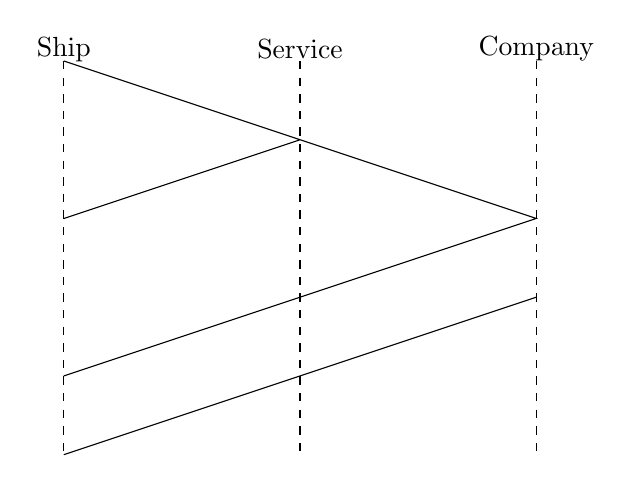
\begin{tikzpicture}
		% timelines
		\draw	[dashed]	(0,5)	--	(0,0)
				[dashed]	(3,5)	--	(3,0)
				[dashed]	(6,5)	--	(6,0);
		% labels
		\draw	(0,5.15)	node	{Ship}
				(3,5.15)	node	{Service}
				(6,5.15)	node	{Company};
		% interaction lines
		\draw	(0,5)	--	(3,4)	--	(0,3)				% API call (request/response)
				(3,4)	--	(6,3)	--	(3,2)	--	(0,1)	% Service requests/recieves data from company/data center
				(6,2)	--	(3,1)	--	(0,0);				% Additional line
	\end{tikzpicture}
	\caption{Rough draft of a model example, where a ship requests something from a service (could be a weather update).}
	\label{fig:modelExProtocol}
\end{figure}
\begin{figure}
	\centering
	\begin{tikzpicture}[->,>=stealth', node distance=3.5 cm, thick]
		\tikzstyle{every state}=[draw=black,rectangle,rounded corners]

		\node[state, initial]	(A)	[]					{No map loaded};
		\node[state]			(B)	[below left of=A]	{Awaiting Map};
		\node[state]			(C)	[below right of=A]	{Map loaded};

		\path	(A)	edge[bend right,left]									node{Request Map}	(B)
					edge[loop above,left,		out=130,in=100,	looseness=7]node{Trash Map}		(A)
				(B)	edge[loop above,below left,	out=130,in=100, looseness=7]node{Request Map}	(B)
					edge[loop below,below,		out=240,in=270, looseness=7]node{Trash Map}		(B)
					edge[bend right,below]									node{Await Response}(C)
				(C)	edge[bend right,above]									node{Request Map}	(B)
					edge[bend right,right]									node{Trash Map}		(A);
	\end{tikzpicture}
	\caption{Final state machine, describing the \ttt{Ship} entity in Figure \ref{tab:fsmEx}.}
	\label{fig:fsmExShip}
\end{figure}

\begin{figure}
	\centering
	\begin{tikzpicture}[->,>=stealth', node distance=3.5 cm, thick]
		\tikzstyle{every state}=[draw=black,rectangle,rounded corners]

		\node[state, initial]	(A)	[]				{Idle};
		\node[state]			(B)	[right of=A]	{Active};

		\path	(A)	edge[loop above,left,	align=center,	out=130,in=100,	looseness=7]	node{Process Request\\(Invalid Request)}(A)
					edge[bend left,	above,	align=center]									node{Process Request\\(Valid Request)}	(B)
				(B)	edge[bend left,	below]													node{Respond}							(A);
	\end{tikzpicture}
	\caption{Final state machine, describing the \ttt{Service} entity in Figure \ref{tab:fsmEx}.}
	\label{fig:modelExFsm}
\end{figure}

\section{Model-Based testing of MCP} 
\TODO{Hvad kan man teste med dette?}

\section{Summary: advantages and disadvantages} 

Issues will inevitably present themselves with a project such as this, however the scope and nature of these issues will vary with each approach possible. As different approaches offer tailored advantages to circumvent correlating unique concerns, another set of unique concerns will necessarily present themselves. In this section I will sum up the approaches presented throughout Chapter \ref{chp:Analysis}, along with their corresponding arising advantages and disadvantages.
\begin{description}
	\item[Manual model-creation]\ \\
	\tbf{Advantages}
	\begin{itemize}
		\item a
		\item b
		\item c
	\end{itemize}
	\tbf{Disadvantages}
	\begin{itemize}
		\item d
		\item e
	\end{itemize}
	\item[Manual model-creation]\ \\
	\tbf{Advantages}
	\begin{itemize}
		\item f
		\item g
		\item h
	\end{itemize}
	\tbf{Disadvantages}
	\begin{itemize}
		\item i
		\item j
		\item k
	\end{itemize}
\end{description}

\TODO{Problematikker: F.eks at folk, der lægger software op ikke nødvendigvis selv kan lave modellerne/forstå at give argumenterne, der skal bruges til at generere modeller automatisk. Diskuter problematikken om at man gerne vil lave tekniske ting, der skal bruges af ikke-tekniske mennesker}
